% Options for packages loaded elsewhere
% Options for packages loaded elsewhere
\PassOptionsToPackage{unicode}{hyperref}
\PassOptionsToPackage{hyphens}{url}
\PassOptionsToPackage{dvipsnames,svgnames,x11names}{xcolor}
%
\documentclass[
  letterpaper,
  DIV=11,
  numbers=noendperiod]{scrartcl}
\usepackage{xcolor}
\usepackage{amsmath,amssymb}
\setcounter{secnumdepth}{-\maxdimen} % remove section numbering
\usepackage{iftex}
\ifPDFTeX
  \usepackage[T1]{fontenc}
  \usepackage[utf8]{inputenc}
  \usepackage{textcomp} % provide euro and other symbols
\else % if luatex or xetex
  \usepackage{unicode-math} % this also loads fontspec
  \defaultfontfeatures{Scale=MatchLowercase}
  \defaultfontfeatures[\rmfamily]{Ligatures=TeX,Scale=1}
\fi
\usepackage{lmodern}
\ifPDFTeX\else
  % xetex/luatex font selection
\fi
% Use upquote if available, for straight quotes in verbatim environments
\IfFileExists{upquote.sty}{\usepackage{upquote}}{}
\IfFileExists{microtype.sty}{% use microtype if available
  \usepackage[]{microtype}
  \UseMicrotypeSet[protrusion]{basicmath} % disable protrusion for tt fonts
}{}
\makeatletter
\@ifundefined{KOMAClassName}{% if non-KOMA class
  \IfFileExists{parskip.sty}{%
    \usepackage{parskip}
  }{% else
    \setlength{\parindent}{0pt}
    \setlength{\parskip}{6pt plus 2pt minus 1pt}}
}{% if KOMA class
  \KOMAoptions{parskip=half}}
\makeatother
% Make \paragraph and \subparagraph free-standing
\makeatletter
\ifx\paragraph\undefined\else
  \let\oldparagraph\paragraph
  \renewcommand{\paragraph}{
    \@ifstar
      \xxxParagraphStar
      \xxxParagraphNoStar
  }
  \newcommand{\xxxParagraphStar}[1]{\oldparagraph*{#1}\mbox{}}
  \newcommand{\xxxParagraphNoStar}[1]{\oldparagraph{#1}\mbox{}}
\fi
\ifx\subparagraph\undefined\else
  \let\oldsubparagraph\subparagraph
  \renewcommand{\subparagraph}{
    \@ifstar
      \xxxSubParagraphStar
      \xxxSubParagraphNoStar
  }
  \newcommand{\xxxSubParagraphStar}[1]{\oldsubparagraph*{#1}\mbox{}}
  \newcommand{\xxxSubParagraphNoStar}[1]{\oldsubparagraph{#1}\mbox{}}
\fi
\makeatother


\usepackage{longtable,booktabs,array}
\usepackage{calc} % for calculating minipage widths
% Correct order of tables after \paragraph or \subparagraph
\usepackage{etoolbox}
\makeatletter
\patchcmd\longtable{\par}{\if@noskipsec\mbox{}\fi\par}{}{}
\makeatother
% Allow footnotes in longtable head/foot
\IfFileExists{footnotehyper.sty}{\usepackage{footnotehyper}}{\usepackage{footnote}}
\makesavenoteenv{longtable}
\usepackage{graphicx}
\makeatletter
\newsavebox\pandoc@box
\newcommand*\pandocbounded[1]{% scales image to fit in text height/width
  \sbox\pandoc@box{#1}%
  \Gscale@div\@tempa{\textheight}{\dimexpr\ht\pandoc@box+\dp\pandoc@box\relax}%
  \Gscale@div\@tempb{\linewidth}{\wd\pandoc@box}%
  \ifdim\@tempb\p@<\@tempa\p@\let\@tempa\@tempb\fi% select the smaller of both
  \ifdim\@tempa\p@<\p@\scalebox{\@tempa}{\usebox\pandoc@box}%
  \else\usebox{\pandoc@box}%
  \fi%
}
% Set default figure placement to htbp
\def\fps@figure{htbp}
\makeatother


% definitions for citeproc citations
\NewDocumentCommand\citeproctext{}{}
\NewDocumentCommand\citeproc{mm}{%
  \begingroup\def\citeproctext{#2}\cite{#1}\endgroup}
\makeatletter
 % allow citations to break across lines
 \let\@cite@ofmt\@firstofone
 % avoid brackets around text for \cite:
 \def\@biblabel#1{}
 \def\@cite#1#2{{#1\if@tempswa , #2\fi}}
\makeatother
\newlength{\cslhangindent}
\setlength{\cslhangindent}{1.5em}
\newlength{\csllabelwidth}
\setlength{\csllabelwidth}{3em}
\newenvironment{CSLReferences}[2] % #1 hanging-indent, #2 entry-spacing
 {\begin{list}{}{%
  \setlength{\itemindent}{0pt}
  \setlength{\leftmargin}{0pt}
  \setlength{\parsep}{0pt}
  % turn on hanging indent if param 1 is 1
  \ifodd #1
   \setlength{\leftmargin}{\cslhangindent}
   \setlength{\itemindent}{-1\cslhangindent}
  \fi
  % set entry spacing
  \setlength{\itemsep}{#2\baselineskip}}}
 {\end{list}}
\usepackage{calc}
\newcommand{\CSLBlock}[1]{\hfill\break\parbox[t]{\linewidth}{\strut\ignorespaces#1\strut}}
\newcommand{\CSLLeftMargin}[1]{\parbox[t]{\csllabelwidth}{\strut#1\strut}}
\newcommand{\CSLRightInline}[1]{\parbox[t]{\linewidth - \csllabelwidth}{\strut#1\strut}}
\newcommand{\CSLIndent}[1]{\hspace{\cslhangindent}#1}



\setlength{\emergencystretch}{3em} % prevent overfull lines

\providecommand{\tightlist}{%
  \setlength{\itemsep}{0pt}\setlength{\parskip}{0pt}}



 


\KOMAoption{captions}{tableheading}
\makeatletter
\@ifpackageloaded{caption}{}{\usepackage{caption}}
\AtBeginDocument{%
\ifdefined\contentsname
  \renewcommand*\contentsname{Table of contents}
\else
  \newcommand\contentsname{Table of contents}
\fi
\ifdefined\listfigurename
  \renewcommand*\listfigurename{List of Figures}
\else
  \newcommand\listfigurename{List of Figures}
\fi
\ifdefined\listtablename
  \renewcommand*\listtablename{List of Tables}
\else
  \newcommand\listtablename{List of Tables}
\fi
\ifdefined\figurename
  \renewcommand*\figurename{Figure}
\else
  \newcommand\figurename{Figure}
\fi
\ifdefined\tablename
  \renewcommand*\tablename{Table}
\else
  \newcommand\tablename{Table}
\fi
}
\@ifpackageloaded{float}{}{\usepackage{float}}
\floatstyle{ruled}
\@ifundefined{c@chapter}{\newfloat{codelisting}{h}{lop}}{\newfloat{codelisting}{h}{lop}[chapter]}
\floatname{codelisting}{Listing}
\newcommand*\listoflistings{\listof{codelisting}{List of Listings}}
\makeatother
\makeatletter
\makeatother
\makeatletter
\@ifpackageloaded{caption}{}{\usepackage{caption}}
\@ifpackageloaded{subcaption}{}{\usepackage{subcaption}}
\makeatother
\usepackage{bookmark}
\IfFileExists{xurl.sty}{\usepackage{xurl}}{} % add URL line breaks if available
\urlstyle{same}
\hypersetup{
  pdftitle={Planet Four: Inter- and Intra-annual Variability of Dark Regolith on Ice Coverage at the Martian South Polar Region},
  pdfauthor={Michael Aye},
  colorlinks=true,
  linkcolor={blue},
  filecolor={Maroon},
  citecolor={Blue},
  urlcolor={Blue},
  pdfcreator={LaTeX via pandoc}}


\title{Planet Four: Inter- and Intra-annual Variability of Dark Regolith
on Ice Coverage at the Martian South Polar Region}
\author{Michael Aye}
\date{2026-03-17}
\begin{document}
\maketitle
\begin{abstract}
A short overview of the Planetary Research done via Citizen Science,
followed by an in-depth review of the Planet Four Citizen Science
projects.
\end{abstract}


\section{Planet Four project}\label{planet-four-project}

\subsection{Science case}\label{science-case}

\subsection{Science case}\label{science-case-1}

\subsection{Science case temporal}\label{science-case-temporal}

\subsection{Science case: Kieffer
model}\label{science-case-kieffer-model}

\pandocbounded{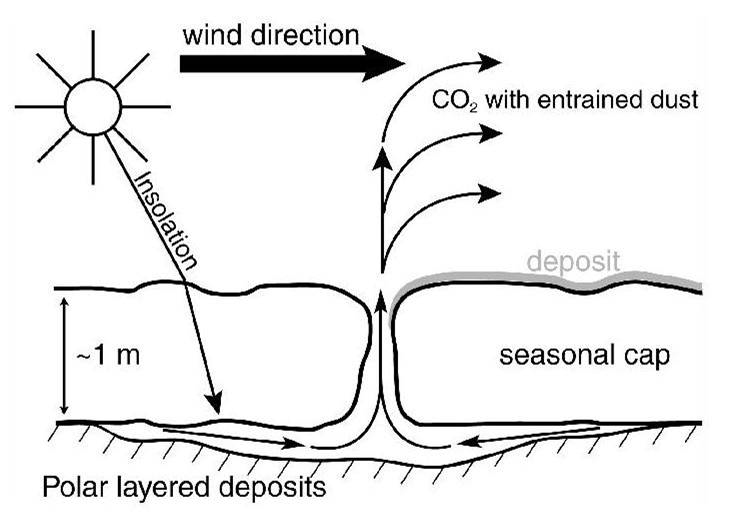
\includegraphics[keepaspectratio]{./image14.jpeg}}

\begin{itemize}
\tightlist
\item
  Jet deposits are aligned by prevalent winds at the time!
\item
  Mapping these features enables the first large area knowledge of
  prevailing winds on Mars!

  \begin{itemize}
  \tightlist
  \item
    on intra-seasonal timescales, not only over many years.
  \end{itemize}
\end{itemize}

\subsection{Active areas around south
pole}\label{active-areas-around-south-pole}

\pandocbounded{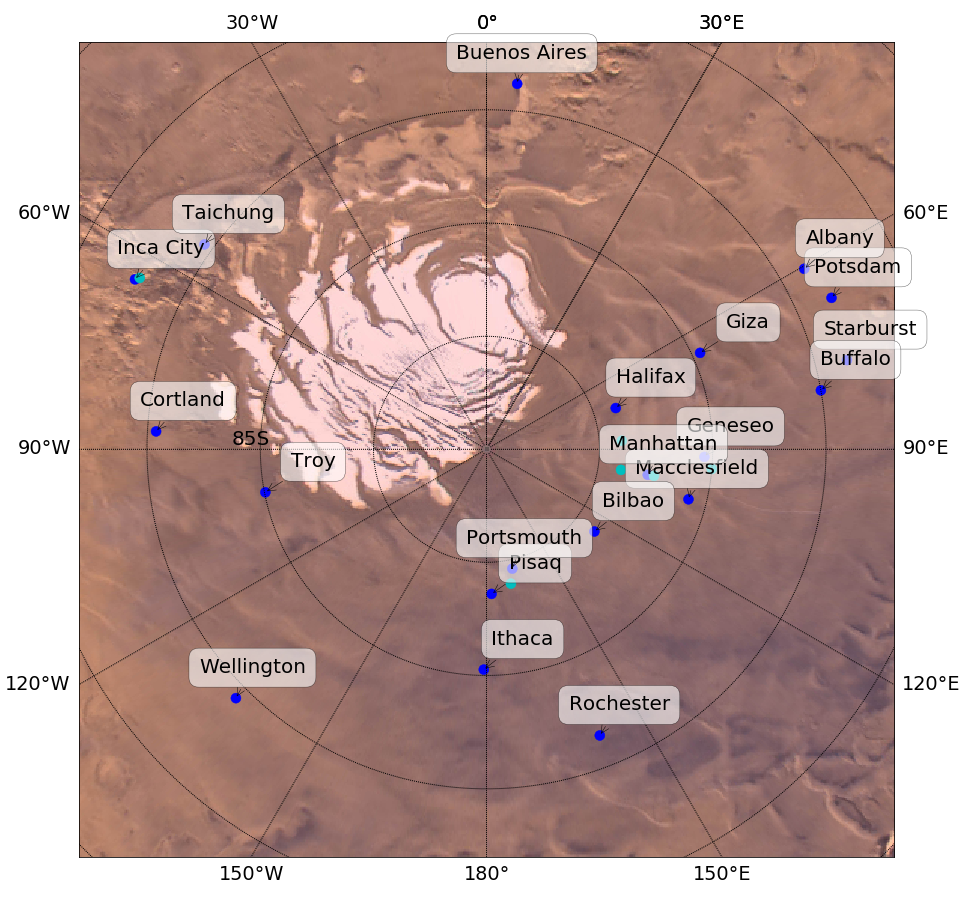
\includegraphics[keepaspectratio]{./rois_map.png}}

\begin{itemize}
\tightlist
\item
  Seasonal campaigns at most of these areas!

  \begin{itemize}
  \tightlist
  \item
    -\textgreater{} Lots of huge HiRISE image data
  \end{itemize}
\end{itemize}

\subsection{Input data}\label{input-data}

\begin{itemize}
\tightlist
\item
  221 HiRISE images from MY 29/30

  \begin{itemize}
  \tightlist
  \item
    new catalog: 469 studied images from MY 28-33 (6 years of data)
  \end{itemize}
\item
  split up into over 30,000 image screen-sized tiles

  \begin{itemize}
  \tightlist
  \item
    now over 64,000 tiles
  \end{itemize}
\item
  Tiles are being ``anonymized'', to prevent bias
\item
  The data input and reduction pipelines need to track everything
\end{itemize}

\subsection{Interface}\label{interface}

\subsection{Interface return}\label{interface-return}

\begin{figure}[H]

{\centering \pandocbounded{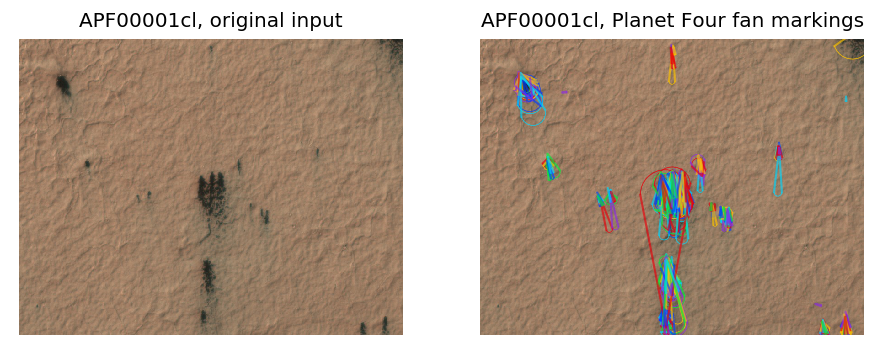
\includegraphics[keepaspectratio]{fan_markings.png}}

}

\caption{Difficulty: What (contrast) defines the ``end'' of a surface
feature?}

\end{figure}%

Minimum of 30 different volunteers per image tile!

=\textgreater{} quite slow progress

\subsection{Reduction pipeline}\label{reduction-pipeline}

\begin{figure}[H]

{\centering \pandocbounded{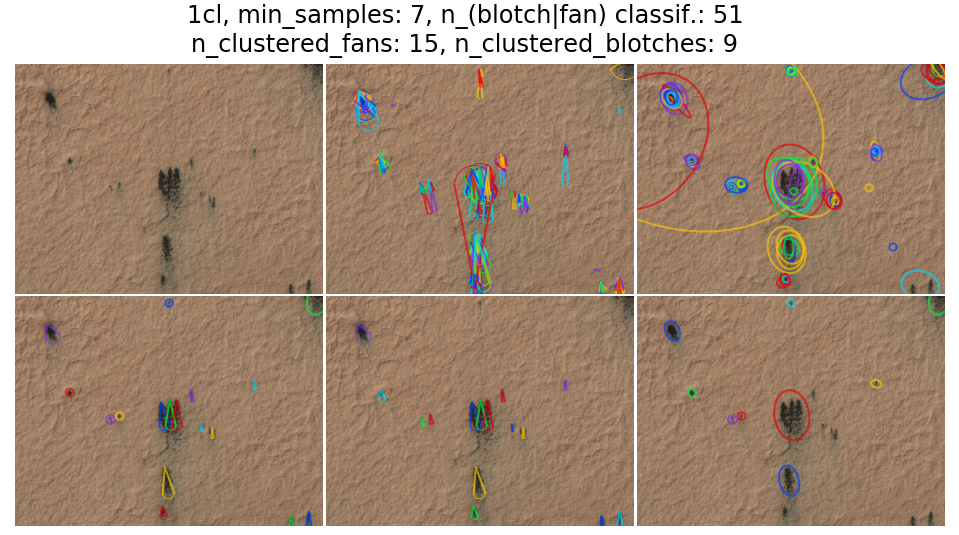
\includegraphics[keepaspectratio]{image23.png}}

}

\caption{Clockwise from upper left: 1) Raw, 2) Fan markings, 3) Blotch
markings, 4) Blotch reduction, 5) Fan reduction, 6) catalog entry with
50\% majority vote}

\end{figure}%

\subsection{Catalog entries}\label{catalog-entries}

\pandocbounded{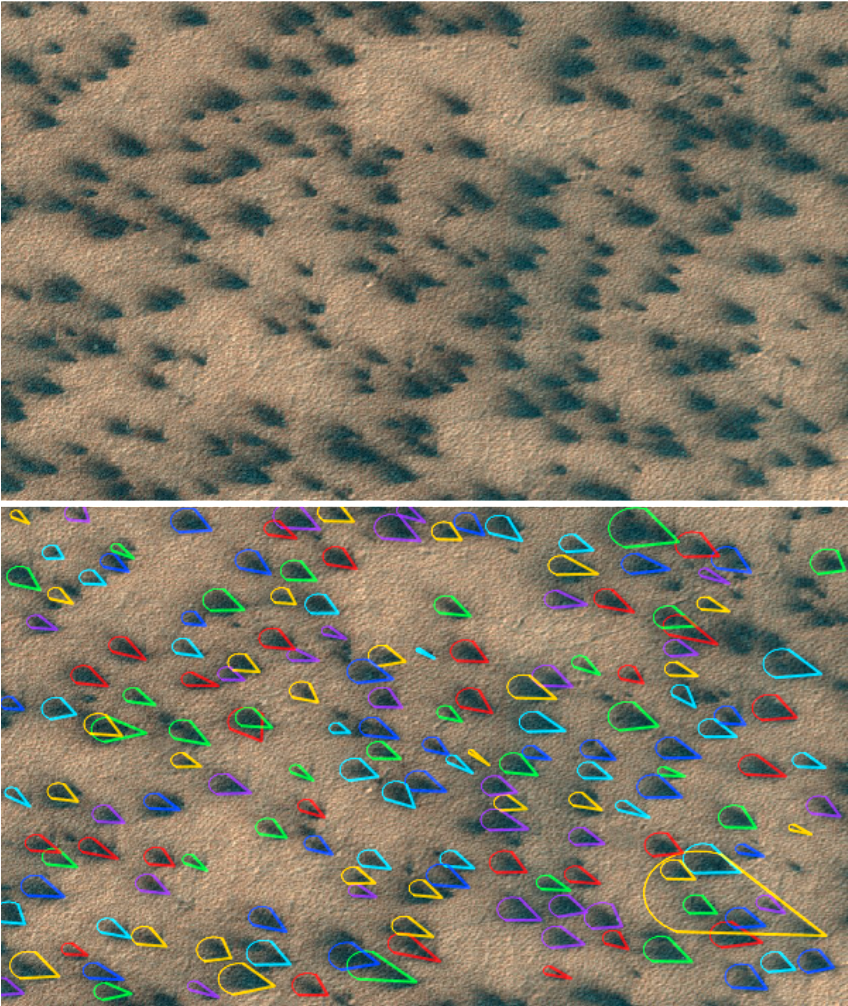
\includegraphics[keepaspectratio]{./image7.png}}
\pandocbounded{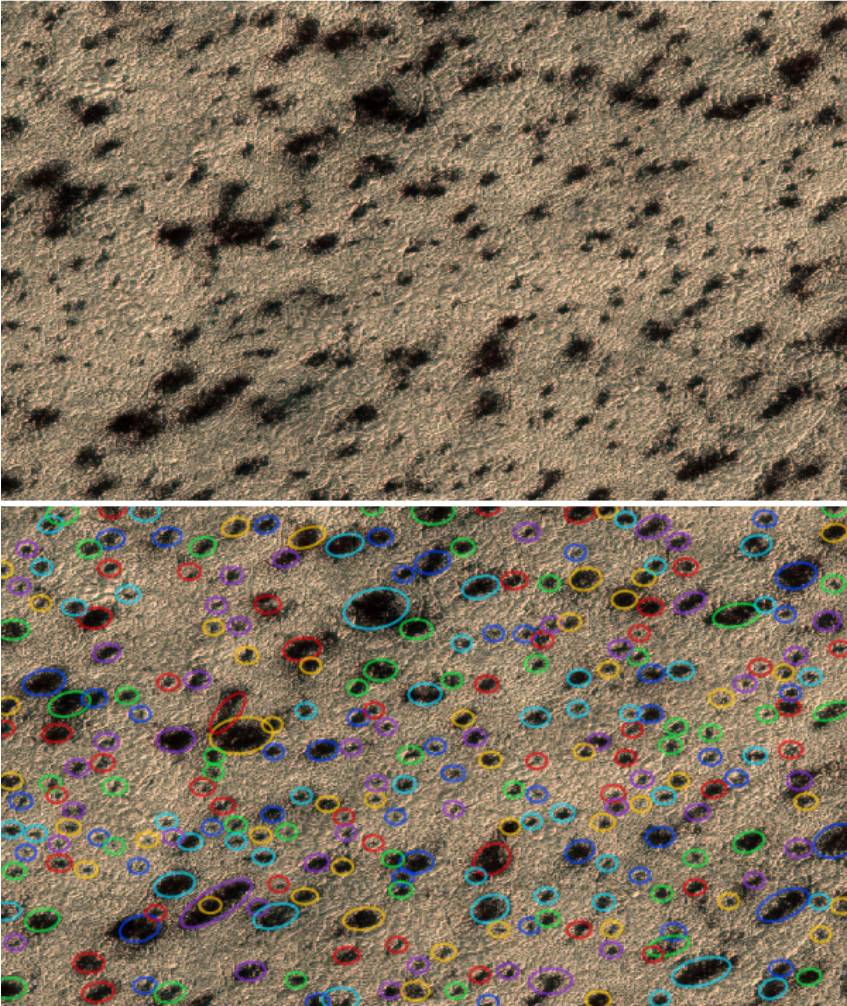
\includegraphics[keepaspectratio]{./image8.png}}

\subsection{Results}\label{results}

\begin{itemize}
\tightlist
\item
  Over 40,000 citizens have contributed

  \begin{itemize}
  \tightlist
  \item
    Most only once
  \item
    Core team of approx 10-20 volunteers did most of the work
  \end{itemize}
\item
  now over 690,000 geo-located objects in catalog
\item
  available at zenodo ``Planet Four Data Catalog'' and via Python
  library ``p4tools''
\end{itemize}

\subsection{What can be done with it?}\label{what-can-be-done-with-it}

\begin{figure}[H]

{\centering \pandocbounded{\includegraphics[keepaspectratio]{image13.gif}}

}

\caption{Portyankina et al. (2022) ``Planet Four: Derived South Polar
Martian Winds Interpreted Using Mesoscale Modeling''}

\end{figure}%

\subsection{Covered surface interests}\label{covered-surface-interests}

\begin{itemize}
\tightlist
\item
  Seasonal CO2 ice is quite bright
\item
  So, how much is covered by dark regolith?
\item
  -\textgreater{} energy balance of the surface and lower atmosphere
\item
  Previous work estimated 20-30\% coverage, but only for a few locations
  and times
\end{itemize}

\subsection{Surface coverage across
years}\label{surface-coverage-across-years}

\pandocbounded{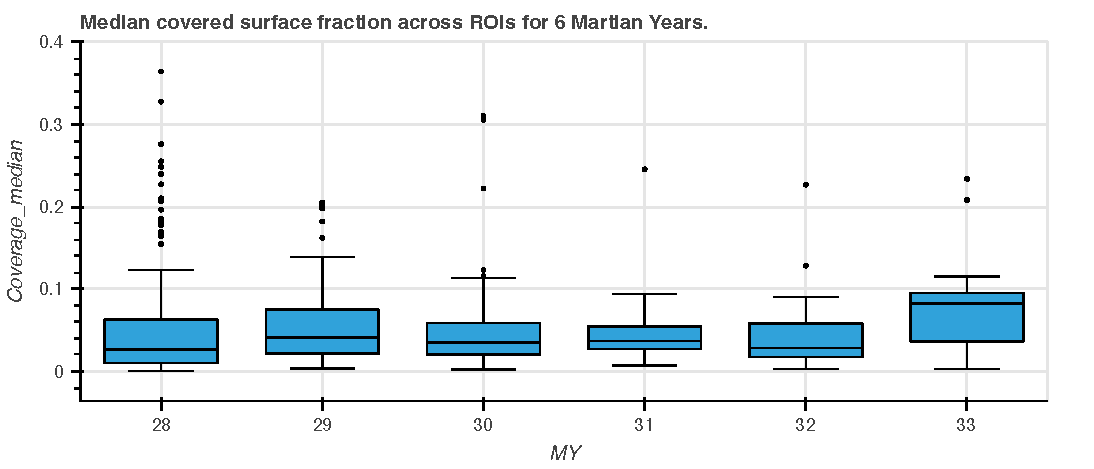
\includegraphics[keepaspectratio]{index_files/mediabag/coverage_across_MY.pdf}}

\subsection{Relationship to global dust
storms?}\label{relationship-to-global-dust-storms}

\pandocbounded{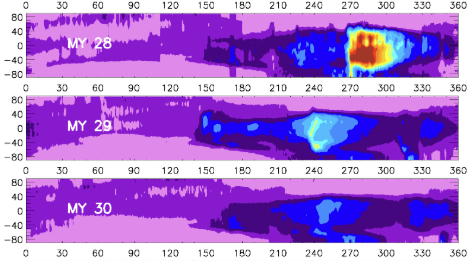
\includegraphics[keepaspectratio]{dust_28_to_30.png}}
\pandocbounded{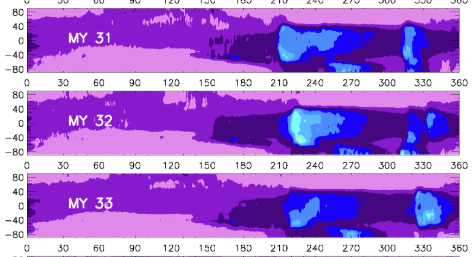
\includegraphics[keepaspectratio]{dust_31_to_33.png}}
\pandocbounded{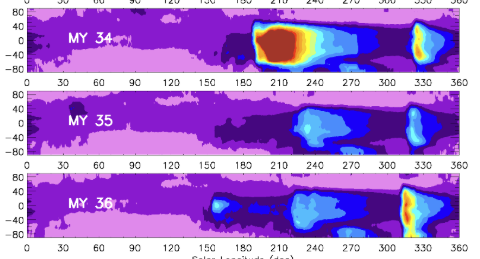
\includegraphics[keepaspectratio]{dust_34_to_36.png}}

\subsection{Intra-seasonal
variability}\label{intra-seasonal-variability}

\pandocbounded{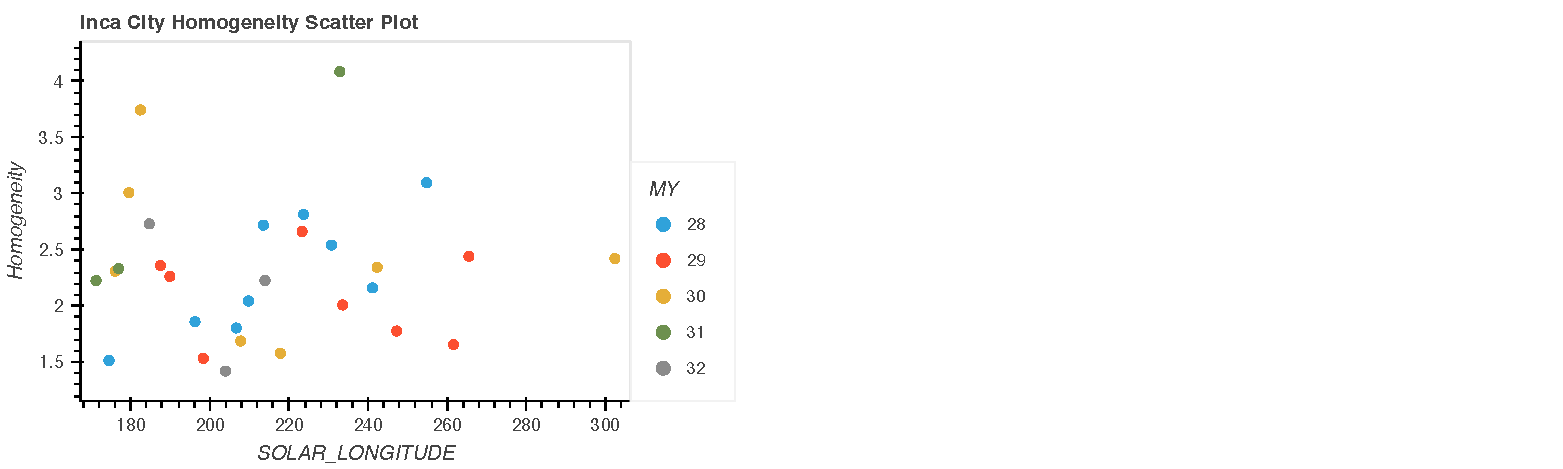
\includegraphics[keepaspectratio]{index_files/mediabag/Inca_City_Homogeneity.pdf}}
\pandocbounded{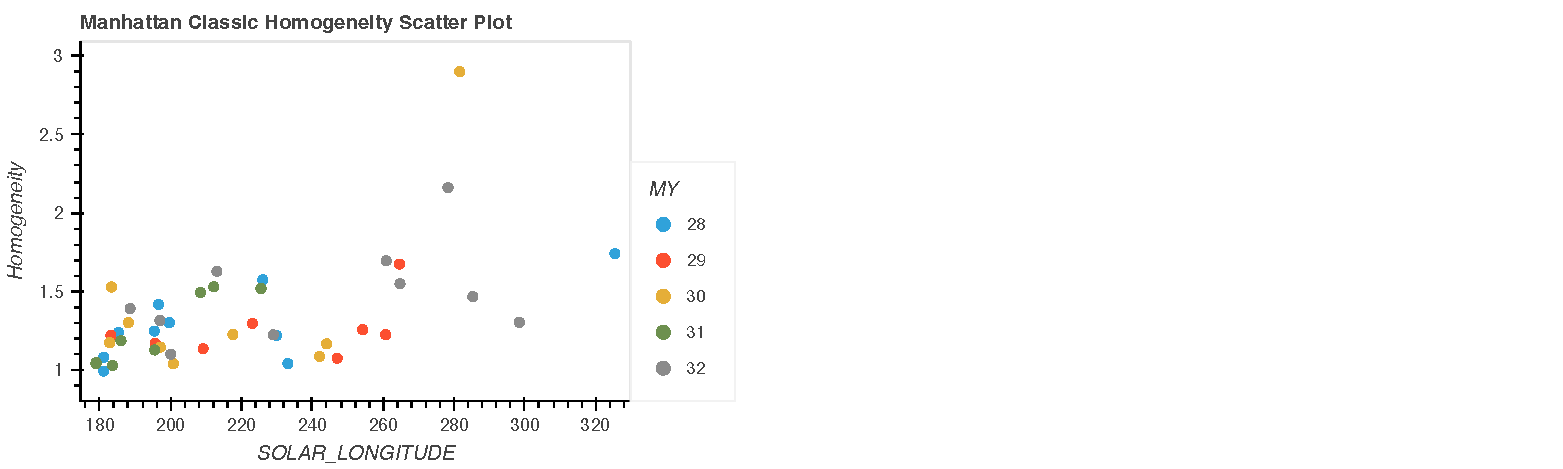
\includegraphics[keepaspectratio]{index_files/mediabag/Manhattan_Classic_Homogeneity.pdf}}

\subsection{Fan lengths}\label{fan-lengths}

Combo of jet and wind strengths

\pandocbounded{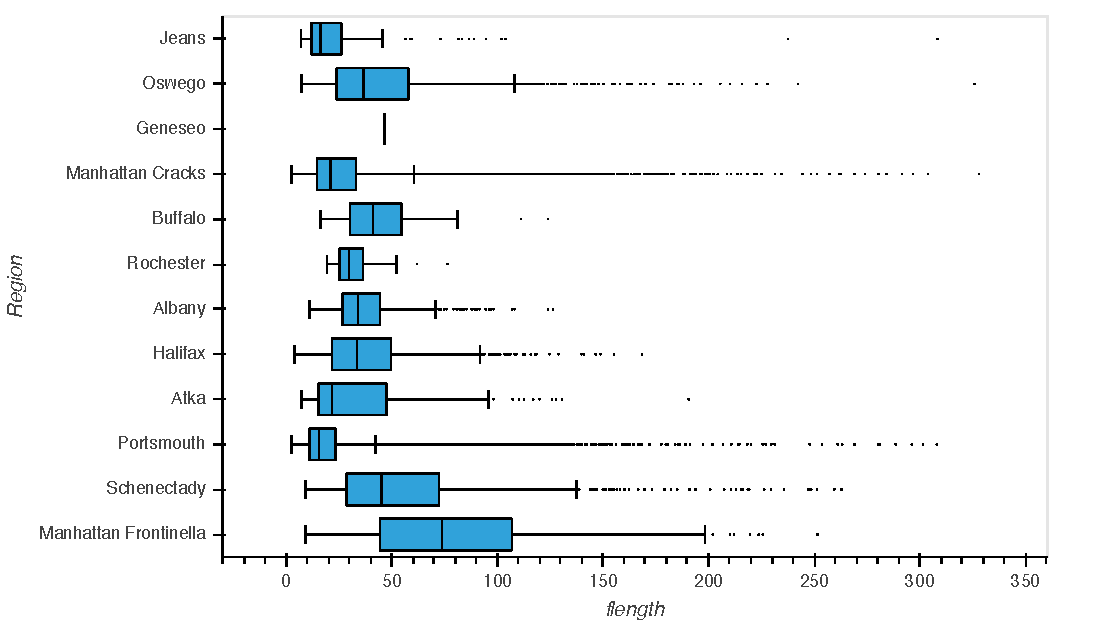
\includegraphics[keepaspectratio]{index_files/mediabag/flength_second.pdf}}

\section{Conclusions}\label{conclusions}

\begin{itemize}
\tightlist
\item
  Surface coverage is very repeatable across years, but varies between
  ROIs
\item
  Relationship to global dust storms is being investigated
\item
  Surface coverage median fractions around 5 \%.
\end{itemize}

\section*{References}\label{references}
\addcontentsline{toc}{section}{References}

\phantomsection\label{refs}
\begin{CSLReferences}{1}{0}
\bibitem[\citeproctext]{ref-portyankinaPlanetFourDerived2022}
Portyankina, Ganna, Timothy I Michaels, Klaus-Michael Aye, Megan E
Schwamb, Candice J Hansen, and Chris J Lintott. 2022. {``Planet {Four}:
{Derived South Polar Martian Winds Interpreted Using Mesoscale
Modeling}.''} \emph{Planet. Sci. J.} 3 (2): 31.
\url{https://doi.org/10.3847/PSJ/ac3087}.

\end{CSLReferences}




\end{document}
